\chapter{Identification du sens du résultat}
\label{chap:sensresultat}


%Hypothèse: Les documents à une seule demande de c sont tellement nombreux que si un doc n'a qu'une seule demande on peut identifier par classification le sens du résultat sur cette demande.
%
%Démonstration: 
%
%- Nb de doc à 1 dmd: si on projette la distribution des demandes dans les docs annotées, sur le corpus plus large, il est fort probable que les les doc à une demande soit majoritaires
%
%- reconnaissance des docs à 1 dmd:  par classification arbre ou ensemble-SVM à moyenne de probabilités
%
%- identification du sens du résultat: classif arbre ou ensembliste ou Gini-PLS
%
%Confiance dans les résultats (impossible du fait du faible nombre de doc - peut-être sur danais)
%
%http://www.joetsite.com/wp-content/uploads/2018/07/Vol.-72-25-18.pdf
%
%Template \verb=2011 Comparing_Mining_Algorithms_for_Predicting_the_Sev.pdf=

\section{Introduction}
\label{sec:sensresultat:motivation}
Comme le précédent, ce chapitre est relatif à l'extraction de données sur les demandes et résultats correspondants. Cependant, il est question ici d'extraire uniquement le sens du résultat d'une demande connaissant sa catégorie. Cette étude est intéressante parce que le problème devient plus simple. En se passant de la localisation précise de l'énoncé du résultat, l'extraction du sens du résultat peut être formulée comme une tâche de classification de documents. Nous modélisons la tâche comme un problème de classification binaire consistant à entrainer un algorithme à reconnaitre si la demande a été rejetée (sens = rejette) ou acceptée (sens = accepte). Cette modélisation est proposée sur une restriction du problème définie par les postulats \ref{postulat:sens:unedemande} et \ref{postulat:sens:sensbinaire} suivants.

\begin{postulat}\label{postulat:sens:unedemande}
Pour toute catégorie de demande $C$, les documents ne contenant qu'une demande de catégorie $C$ sont majoritaires. %\textcolor{red}{COMMENT SAVOIR QU'UN DOCUMENT N'A QU'UNE SEULE DEMANDE? CLASSIFICATION POSSIBLE?}
%Pour toute catégorie de demande $C$, on ne considère que les décisions dans lesquelles n'apparaît qu'une seule demande de catégorie $C$. 
\end{postulat} 
Ce postulat est légitime car les statistiques sur les données labellisées de la Figure \ref{fig:quanta:hist-repartition-docs} montrent bien que dans chaque catégorie, les décisions contiennent en majorité une demande. On remarque néanmoins l'exception de la catégorie STYX (dommage-intérêt sur l'article 700 CPC), où dans la majorité des documents, on a plutôt 2 demandes. Cette exception peut se justifier par le fait que chaque partie fait généralement ce type de demande car elle porte sur le remboursement des frais de justice. Ce postulat présente cependant un inconvénient dû au fait que la majorité des demandes se trouvent dans des décisions à plus d'une demande. Il est donc possible de manquer un grand nombre de demandes. %On pourrait peut-être porter la classification à un modèle multi-label qui déterminera plusieurs sens à partir d'un seul document. Par exemple <SENS1, SENS2, SENS3> avec des valeurs prédéfinies sur les SENS 2 et 3 par exemple NO-DMD pour indiquer que la décision ne comprend pas de seconde ou de troisième demande.

\begin{postulat}\label{postulat:sens:sensbinaire}
Le sens du résultat est généralement binaire: accepte ou rejette.
\end{postulat} 
Ce postulat est justifié car les sens de résultat ont majoritairement l'une de ces deux valeurs (Figure \ref{stat-sensrst}). Les autres sens sont très rares.

\begin{figure}
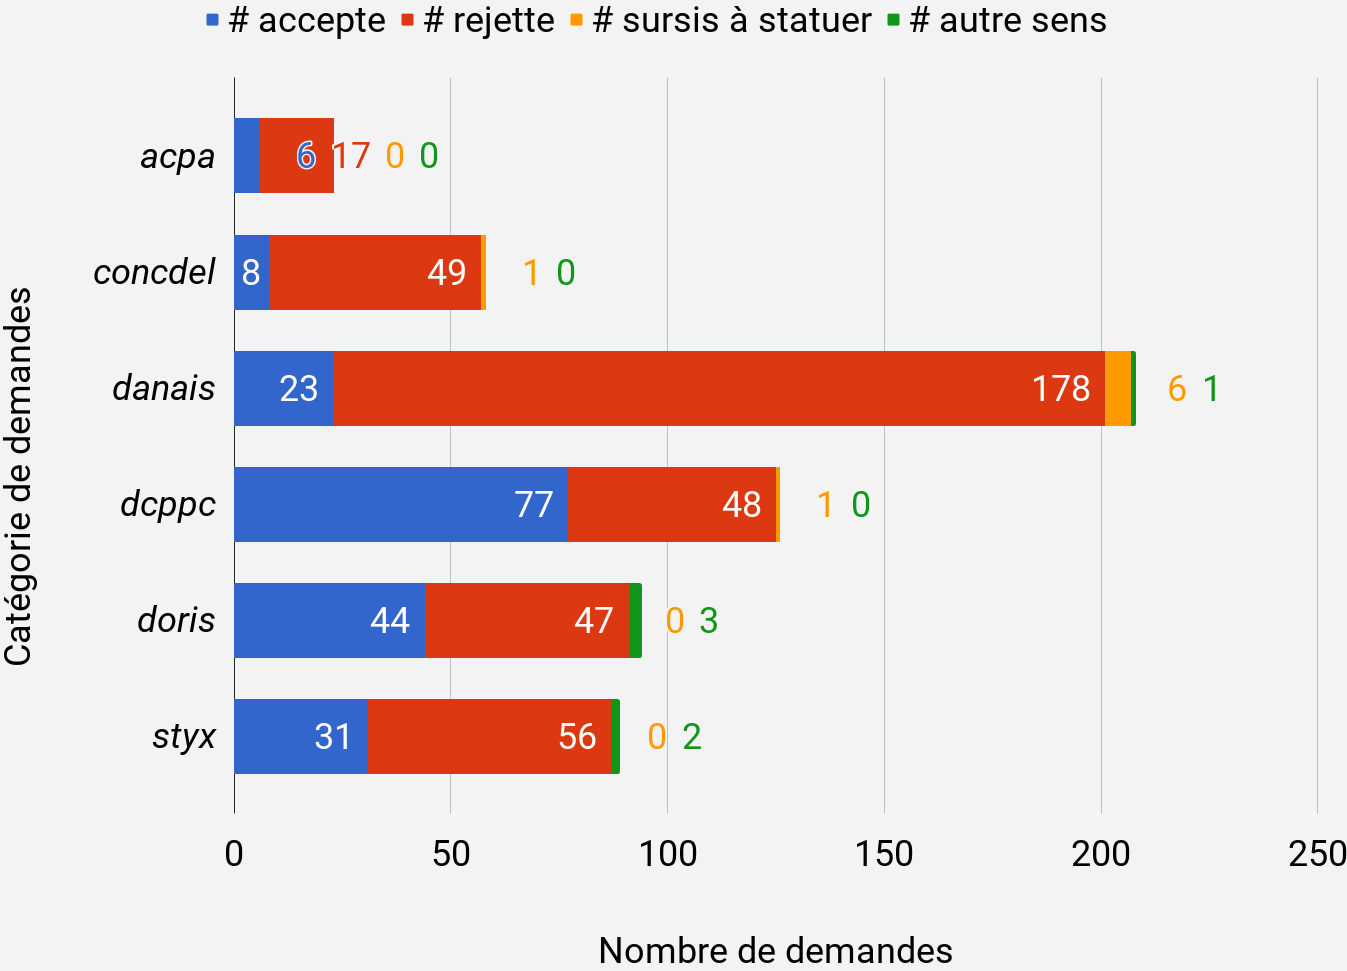
\includegraphics[width=\textwidth]{chartDistrSens.png}
\caption{Répartition des sens de résultat dans les données annotées.}\label{stat-sensrst}
\end{figure}

Cette étude porte sur l'analyse de l'impact de différents aspects techniques généralement impliqués dans la classification de textes qui consistent en général à une combinaison de représentations des documents et d'algorithmes de classification. Cette analyse permettra de savoir s'il existe une certaine configuration permettant de déterminer le sens du résultat à une demande sans identifier précisément cette dernière dans le document. 


\section{Classification de documents}
\label{sec:sensresultat:biblio_classif}

La classification de textes permet d'organiser des documents dans des groupes prédéfinis. Elle reçoit depuis longtemps beaucoup d'attentions. Deux choix techniques influencent principalement les performances: la représentation des textes et l'algorithme de classification. Dans la suite, la variable à prédire est notée $y$, et la base d'apprentissage comprend les observations de l'échantillon $S = \lbrace (x_i, y_i)_{i=1..n} \rbrace$.

\subsection{Algorithmes traditionnels de classification de données}
Bien que la classification de documents voit se développer récemment des algorithmes propres aux textes, un grand nombre de méthodes ont été développées. Ces méthodes sont généralement basée sur une représentation  des textes dans un espace vectoriel $\mathcal{X}$ d'entrée et délimitent une frontière entre les classes dans un espace multidimensionnel. Les notations du Tableau \ref{tab:quanta:notations_metriques} sont utilisées dans cette section. 
%NB et SVM : https://www.dropbox.com/home/Documents/to-read/term-weight?preview=Best+Terms+An+Efficient+Feature+Selection+Algorithm+for+Text+Categorization.pdf
% C4.5, k-means, svm, apriori algo, em algo, page rank, ada boost, knn, NB, CART: http://www.cs.umd.edu/~samir/498/10Algorithms-08.pdf

\subsubsection{Le Bayésien naïf (NB)}
%http://stackoverflow.com/questions/10059594/a-simple-explanation-of-naive-bayes-classification#20556654
%https://webdocs.cs.ualberta.ca/~greiner/R/PAPERS/ExplainNB.pdf
Le classifieur naïf bayésien \citep{duda1973patternclass} est  un modèle à densité qui estime la probabilité qu'un texte appartienne à une classe à l'aide du théorème de Bayes \citep{raschka2014naivebayes}:
\begin{equation}
\text{probabilité a posteriori} = \frac{\text{probabilité conditionnelle} \cdot \text{probabilité a priori}}{\text{évidence}}
\end{equation}

La probabilité a posteriori peut être interprétée pour la classification de documents par la question "Quelle est la probabilité que le document $d$ soit de la classe $y=c \in C$ ?". La réponse à cette question se formalise comme suit:

\[\p(y=c \vert d) = \frac{\p(d \vert c)\p(c)}{\p(d)}, \forall c \in C \]
ou plus simplement  $\p(y = c \vert d) = \p(c)\p(d \vert c)$ car $\p(d)$ ne change pas en fonction de la classe et peut donc être ignorée \citep{rish2001nb_study}. $d$ est catégorisé dans la classe $c$ pour laquelle $\p(c \vert d)$ est maximale: \[y = \argmax_{c \in C} \p(c \vert d).\]

 La phase d'entrainement, appliquée à des exemples déjà labellisés, permet d'estimer les paramètres $\p(c)$ et $\p(d \vert c)$ qui servent à calculer $\p(c \vert d)$.

$\p(c)$ est estimé par la proportion de documents classés dans $c$ parmi les exemples d'apprentissage: $\p(c_j) = \frac{N_c}{N}, \forall c \in C$.


 $\p(c \vert d)$ est estimé grâce l'hypothèse \ref{hypo:sens_rst:iid} d'{indépendance conditionnelle des descripteurs (termes)}. Une hypothèse naïve dont la violation, par les données réelles, n'empêche pas le NB de bien fonctionner \citep{rish2001nb_study}. 

\begin{hypothese}[indépendance conditionnelle des   descripteurs] [ Un modèle naïf bayésien étant de type génératif], la position de chaque mot dans le texte est générée indépendamment de tout autre mot étant connue la catégorie du texte. \label{hypo:sens_rst:iid}
\end{hypothese}

Si l'ensemble des termes de $d$ est $\lbrace t_{1}, \dots, t_{K} \rbrace$, alors grâce à l'hypothèse \ref{hypo:sens_rst:iid},
$\p(d \vert c) = \p(t_{1}, \dots, t_{K}\vert c) = \prod_{k=1}^K \p(t_{k} \vert c)$, et pour un terme $t_k$, la probabilité conditionnelle $\p(t_k \vert c)$ est la proportion d'exemples de $c$ qui contiennent $t_k$:  $\p(t_k \vert c) = \frac{N_{t_k,c}}{\vert D_c \vert }, \forall k \in \lbrace 1, \dots, K \rbrace$.

\subsubsection{Machine à vecteurs de support (SVM)}
\label{sec:sens-resultat:svm}
La classification binaire par une machine à vecteurs de support (SVM) \citep{vapnik1995statlearning} affecte à tout objet en entrée $x$ la classe $y$ qui correspond au coté d'un hyperplan, séparant les exemples d'entraînement des classes candidates, où $x$ se trouve. La phase d'apprentissage consiste à déterminer l'hyperplan optimal $w^T x + b = 0$ i.e. dont la marge\footnote{La plus petite distance entre les échantillons d'apprentissage et l'hyperplan séparateur} est maximale (Figure \ref{fig:sensresultat:svm}\footnote{\url{http://web.mit.edu/6.034/wwwbob/svm-notes-long-08.pdf}}).

\begin{figure}[!htb]
	\centering
	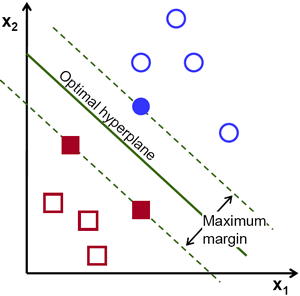
\includegraphics[width=0.5\textwidth]{svm.png}
	\caption{Hyperplan optimal et marge maximale d'un SVM.}\label{fig:sensresultat:svm}
\end{figure}

 Le vecteur  $w$ des  poids des caractéristiques et le biais $b$ sont déterminés par le problème d'optimisation du \og SVM à marges molles \fg{} de \citet{Cortes1995svm} :
 

\begin{equation*}
\begin{aligned}
& \min\limits_{w,b}
& &\frac{1}{2}\norm{w}^2 + C \sum\limits^n_{i=1} \xi_i \\
& \text{s.c.}
& & y_i(w^T+b)\geq 1-\xi_i, \xi_i \geq 0.
\end{aligned}
\end{equation*}

où $C$ est la constante de régularisation pour éviter un sur-apprentissage ou le sous-apprentissage, les $\xi_i$ sont des variables ressort (\textit{slack variables}) qui permettent à des points de se retrouver dans la marge. 

% variables ressort: https://cours.etsmtl.ca/gti770/private/notes/PDF/LOG770-SVM_1pp.pdf

La classification par SVM ne s'applique que lorsque les exemples d'apprentissage des classes sont linéairement séparables. Cependant, ils ne le sont pas toujours dans l'espace  $\mathcal{X}$. Ainsi, une fonction \og noyau \fg{} (\textit{kernel}) $K: \mathcal{X} \longrightarrow \mathcal{F}$ doit être choisie pour transformer chaque donnée entrée $x$ de l'espace original  $\mathcal{X}$ vers un nouvel espace  $\mathcal{F}$ dit de caractéristiques dans lequel les classes sont linéairement séparables. Par conséquent, la fonction de classification s'écrit \[f(x) = \sum\limits_{i=1}^n \alpha_i K(x,x_i) + b\] où les $\alpha_i$ sont les coefficients de la combinaison linéaire des exemples d'apprentissage égale à $w$ ($w = \sum\limits_{i=1}^n\alpha_i x_i$) \citep{Ben-Hur2010svm}. Parmi les multiples formes qu'il peut prendre, le noyau peut être, par exemple, soit linéaire($K(x,x_i) = x^Tx_i + c$), soit polynomial ($K(x,x_i) = (\gamma x^Tx_i + c)^d$), soit Gaussien ou RBF\footnote{\textit{radial base function}} ($K(x,x_i) = \exp{-\gamma \norm{x-x_i}}$), soit une sigmoïde ($K(x,x_i) = \tanh(\gamma x^Tx_i + c)$) \citep{Amami2015PracticalModelSelectionSVM}.

\subsubsection{k-plus-proches-voisins (kNN)}
L'algorithme des $k$-plus-proches-voisins est un algorithme très simple qui consiste à affecter à un nouvel objet la classe majoritaire $y'$ parmi ceux des $k$ points d'exemples d'entrainement $\lbrace (x_i,y_i) \rbrace_{1:k}$, les plus proches du point $x'$ de cet objet selon la métrique $d$ choisie. Ainsi, trois éléments clés influencent l'efficacité de la classification:
\begin{enumerate}
	\item les données d'entrainement dont le nombre s'il est très grand peut rendre cher le processus de classification, car la distance du nouvel objet à chaque point annoté, est calculée;
	\item le nombre de voisins (c'est-à-dire la valeur de $k$) qui ne doit être ni très petit (sensibilité aux bruits / \textit{outliers}), ni très grand (risque d'avoir dans le voisinage beaucoup de points d'une autre classe). La sensibilité au nombre de voisins peut être atténuée en pondérant les points par leur distance à l'objet à classer. Il a été proposé plusieurs variantes de cette stratégie de \og vote pondéré par la distance \fg{}, comme par exemple:
	\begin{itemize}
		\item $y' = \argmax\limits_c \sum\limits_{(x_i,y_i)} \frac{1}{Dis(x', x_i)^2} \times I(c = y_i)$  \citep{dudani1976originalwknn} \[\text{ où } I(c=y_i) = \left\lbrace \begin{array}{ll}
		1 & \text{si }c = y_i \\
		0 & \text{sinon}
		\end{array} \right.\]
		\item $y' = \argmax\limits_c \sum\limits_{(x_i,y_i)} w_i \times I(c = y_i)$ \citep{gou2011wknn} \[\text{ avec } w_i = \left\lbrace \begin{array}{ll}
		\frac{Dis(x, d_k) - Dis(x, d_i)}{Dis(x, d_k) - Dis(x, d_1} & \text{si } Dis(x, d_k) \neq Dis(x, d_1) \\
		1 & \text{sinon}
		\end{array} \right.\]
		%\item $y' = \argmin\limits_c d(vec(\hat{E}(x)),t_c)$ \citep{bicego2016wknnrevisited} avec $\hat{E} = ?$ et $t_c = ?$
	\end{itemize}
	 
	\item la métrique de calcul de distance qui doit être adéquate pour le type de donnée et la tâche, comme par exemple, la distance cosinus qui est préférable à la distance euclidienne pour la classification de documents, la deuxième métrique se dégradant lorsque le nombre d'attributs augmente.
\end{enumerate}

% le KNN souffre de 2 pbs: la complexité et la définition de la distance à utiliser. Le kNN doit stocker et rechercher à travers toute la base d'entraînement pour classer un point (O(n)). La recherche des voisins peut être accélérée en utilisant des algorithmes comme KD-trees\footnote{\url{https://gopalcdas.com/2017/05/24/construction-of-k-d-tree-and-using-it-for-nearest-neighbour-search/}} [Jon Louis Bentley, 1975] (O(k log(n))) ou ball-trees. La construction du kd-tree consiste à diviser les données d'entrainement à chaque  niveau suivant une valeur d'une dimension en essayant d'obtenir un arbre le plus équilibré possible pour optimiser la recherche. Le nombre de dimension doit être assez réduit?????
\subsubsection{Arbre de décision}
Un arbre de décision est une structure arborescente utilisée en fouille de données pour associer un label prédéfini à des objets (classification), ou prédire la valeur d'une variable continue (régression). Il comprend des n\oe{}uds internes qui correspondent chacun à un test sur la valeur d'un attribut (test uni-varié), des arêtes correspondant à une sortie du test, et enfin des feuilles ou n\oe{}uds terminaux qui correspondent chacun à une prédiction. La classification d'un objet $x$ consiste à faire passer successivement les tests en fonction des valeurs des attributs de $x$, de la racine jusqu'à une feuille dont le label est retourné comme classe de $x$ (Algorithme \ref{algo:sensresultat:classifywithtree}).

\begin{algorithm}[ht] \small
	\KwData{Objet $x$, Arbre $A$}
	\KwResult{label}
	$n := racine(A)$ \; 
	\While{$n$ n'est pas une feuille}{
		Effectuer sur $x$ le test associé à $n$\;
		$n :=$ noeud fils de $n$ correspondant au résultat du test \;
	}
	\Return le label associé à la feuille $n$\;
	\caption{Classification par arbre de décision} \label{algo:sensresultat:classifywithtree}
\end{algorithm}

La construction de l'arbre (phase d'apprentissage) consiste à générer une hiérarchie de tests, aussi courte que possible, qui divise successivement l'ensemble $S$ d'exemples d'apprentissage en sous-ensembles disjoints de plus en plus pures\footnote{homogénéité des labels}. %, tels que des sous-groupes de cas appartenant à la même classe soient rapidement détectés. 
L'arbre est construit de la racine aux feuilles en divisant les données d'entraînement $S_{t}$ à chaque nœud ($t$) de sorte à minimiser le degré d'impureté des sous-ensembles d'exemples  $S_{t_i}$ dans les n\oe{}uds fils ($t_i$). Le critère de coupe est généralement défini à partir d'une métrique d'impureté comme par exemple:
\begin{itemize}
	\item l'entropie de la distribution des classes dans $S_t$: \\ $h_C(S_t) = - \sum\limits_{c \in C} \left[p(c \vert S_t) \log_2 p(c \vert S_t)\right];$
	\item l'indice de Gini mesurant la divergence entre les distributions de probabilité des valeurs de la variable prédite: $g_C(S_t) = 1 - \sum\limits_{c \in C} \left[p(c \vert S_t)\right]^2;$
	\item l'erreur de classification définie par : $e_C(S_t) = 1 - \max\limits_{c \in C} \left[p(c \vert S_t)\right]$. 
\end{itemize}
Pour ces métriques, $p(c \vert S_t)$ représente la proportion d'exemples du n\oe{}ud $t$ appartenant à $c$. Parmi les critères de séparation les plus populaires associés à ces métriques d'impureté, on retrouve: 

\begin{itemize}
	\item le gain d'information apporté par le test $t$ portant sur l'attribut $a$ (qui divise $S_t$ en des sous-ensembles $S_{t_i}$) utilisant l'entropie comme métrique d'impureté, et est définie par la différence entre l'entropie de $t$ et l'entropie moyenne des fils de $t$: \\ $ig(S_t, a) = h_C(S_t) - i(S_t, t, a) =  h_C(S_t) - \sum\limits_{S_{t_i}} \frac{\vert S_{t_i} \vert}{\vert S_{t} \vert} \cdot h_C(S_{t_i});$
	\item le rapport des gains, qui corrige le gain d'information, biaisé en faveur des tests ayant un grand nombre d'alternatives (sorties du nœud), en prenant en compte l'information intrinsèque $h_t(S_t)$ de la séparation de $S_t$ suivant le test $t$ en sous-ensembles $S_{t_i}$: \\$gr(S_t, t, a) = \frac{ig(S_t, t, a)}{h_t(S_t)} \text{ avec } h_t(S_t) = \sum\limits_i \frac{\vert S_{t_i}\vert}{\vert S_t \vert} \log_2 \left(\frac{\vert S_{t_i}\vert}{\vert S_t \vert}\right)$
	\item le critère binaire de "doublage" (\textit{twoing criteria}) qui ne s'emploie que pour les arbres binaires : \\ $tc(t) = \frac{P(S_{t_R} \vert S_t)P(S_{t_L} \vert S_t)}{4} \left[\sum\limits_{c \in C} \vert p(c \vert t_L) - p(c \vert t_R)\vert\right]^2$ où  $P(S_{t_R} \vert S_t)$ et $P(S_{t_L} \vert S_t)$ sont les proportions de $S_t$ qui vont respectivement dans les fils $t_R$ et $t_L$ après séparation suivant le test $t$.
\end{itemize}

Les variables nominales peuvent être divisées soit en utilisant autant de partitions que de valeurs distinctes, soit uniquement en des partitions binaires suivant des tests booléens nécessitant de rechercher la division optimale. Les variables numériques sont divisées quant à elles soit par discrétisation de leur domaine en les transformant en variables catégoriques ordinales, soit en recherchant la meilleure division binaire parmi  toutes les séparations possibles. 

La construction de l'arbre est une division récursive qui peut continuer tant qu'il est possible d'améliorer la pureté des nœuds, ce qui peut engendrer un arbre très grand résultant en un sur-apprentissage\footnote{Un modèle trop précis a un très faible taux d'erreur sur les données d'entraînement (erreur d'apprentissage) mais un fort taux d'erreur sur les données de test (erreur de test).}, et une forte complexité temporelle et spatiale lors de la prédiction. Pour s'arrêter plus tôt ("pré-élagage"), plusieurs conditions sont possibles comme par exemple, l'atteinte par la taille des données ($\vert S_t \vert$) d'un seuil minimum, ou l'atteinte par l'arbre d'une profondeur maximale, ou l'amélioration du critère de division est très faible, etc. Le post-élagage\footnote{Suppression de sous-arbres superflus ou en trop après génération de l'arbre.} est appliqué après construction de l'arbre toujours dans le but de minimiser le sur-apprentissage et la complexité. Le post-élagage peut consister par exemple, soit à simplement et rapidement éliminer successivement les feuilles si cela  ne fait pas croître le taux d'erreur sur $S$ (\og élagage basé sur la réduction du taux d'erreur \fg{}), et remplacer chaque nœud par sa classe majoritaire, soit à éliminer successivement les sous-arbres qui minimisent $\frac{erreur(elagage(A, A'), S) - erreur(A, S)}{\norm{feuille(A)} - \norm{feuille(elagage(A, A'))}}$ (\og stratégie coût-complexité \fg{}). 

Les algorithmes de construction d'arbres diffèrent ainsi par leur critère de séparation, leur stratégie d'élagage, et leur capacité à gérer les types d'attributs, les valeurs manquantes et extrêmes. \citet{singh2014id3cartc45} comparent les deux algorithmes CART \citep{Breiman1984CART} (critère de \og doublabe \fg{}, élagage coût-complexité) et C4.5 \citep{quinlan1993c4.5} (rapport des gains, élagage à réduction d'erreur).

\subsubsection{Analyses discriminantes linéaires et quadratiques}
\textcolor{red}{Pas de citation?}
L'analyse discriminante comprend l'ensemble des méthodes déterminant les combinaisons linéaires de variables qui permettent de séparer le mieux possible $K$ catégories ou variables qualitatives. Les analyses linéaires et quadratiques sont des méthodes probabilistes basées sur la probabilité conditionnelle d'appartenance d'un objet $X$ à une classe $y_k$: \[P(Y=y_k \vert X) = \frac{P(Y=y_k) P(X \vert Y=y_k)}{P(X)} = \frac{P(Y=y_k) P(X \vert Y=y_k)}{\sum\limits_{j = 1}^K P(Y=y_j) P(X \vert Y=y_j)}.\]
La classe de $X$ est donc $y_{k*} = \argmax_k P(Y=y_k \vert X) = P(Y=y_k) P(X \vert Y=y_k)$ car le dénominateur est le même pour toutes les classes. Dans cette expression, $P(Y=y_k)$ est la proportion d'exemples de classes $y_k$ dans l'ensemble des données d'apprentissage. Il ne reste donc qu'à déterminer $P(X \vert Y=y_k)$, pour trouver $y$. Deux hypothèses simplifient les calculs:
\begin{enumerate}
	\item l'hypothèse de normalité statuant que la probabilité conditionnelle $P(X \vert Y)$ suit une loi normale multivariée: \[P(X \vert Y = y_k) = \frac{1}{\sqrt{2\pi det(V_k)}}e^{-\frac{1}{2}(X - \mu_k)'V_k^{-1}(X - \mu_k)} \] $\mu_k$ étant le centre de gravité conditionnel, et $V_k$ la matrice de variance covariance conditionnelle;
	\item l'hypothèse d'homoscédasticité statuant que les matrices de variance co-variance conditionnelles sont identiques i.e.: \[\forall j, k \in \lbrace 1,...,K \rbrace, V_j = V_k = V.\]
\end{enumerate}

L'analyse discriminante linéaire (LDA) est définie par une simplification de $P(X \vert y_k)$ sous ces deux hypothèses. En effet, grâce à la proportionnalité de la probabilité conditionnelle à :$\ln\left[P(X \vert y_k)\right] \propto -\frac{1}{2}( X - \mu_k )'V^{-1}(X - \mu_k )$\textcolor{red}{(Vérifier la position de la transposée)}, on déduit une fonction discriminante (ou de classement) linéaire proportionnelle à $P(y_k \vert X)$: \[d(y_k, X) = \ln\left[P(Y = y_k)\right] + \mu_k V^{-1}X' - \frac{1}{2}\mu_k V^{-1}\mu_k'.\] Ainsi $y_{k*} = \argmax_{k \in \lbrace 1,...,K \rbrace} d(y_k, X)$.

L'analyse discriminante quadratique (QDA) considère l'hétéroscédasticité (i.e. $\exists k \neq j, V_k \neq V_j$), et donc ne s'appuie que sur la 1e hypothèse (multinormalité). Dans ce cas, on obtient une règle quadratique de classification $k* = \argmax_{k \in \lbrace 1,...,K \rbrace} Q_k(X)$ où:
\[Q_k(X) = (X - \mu_k)' V_k^{-1}(X - \mu_k) - 2 \ln(\pi_k) + \ln(det(V_k))\] est la fonction quadratique de classement de la classe $k$.

%\subsubsection{Modèles ensemblistes}


\subsection{Algorithmes dédiés aux textes}
Les algorithmes dédiés aux textes intègrent leur propre représentation de document, contrairement aux algorithmes opérant dans des espaces vectoriels aux axes et poids paramétrables à volonté comme le SVM.  Actuellement, les algorithmes NBSVM \citep{wang2012nbsvm} et FastText \citep{grave2017fasttextcls} sont les plus populaires pour la classification de documents avec une très bonne précision pour l'analyse de sentiments \textcolor{red}{[citation]}. 


\subsubsection{NBSVM}

Le NBSVM \citep{wang2012nbsvm} est un classifieur binaire (deux labels $\lbrace -1; 1 \rbrace$) dont le principe consiste à transformer les poids $f^{(k)}$ caractéristiques $V$ des textes $x^{(k)}$, réduits à leur simple présence $\widehat{f}^{(k)}$ en réalisant leur produit élément à élément ($\overset{\sim}{f}^{(k)} = {r} \circ \widehat{f}^{(k)}$) avec le vecteur de poids $r$ du classifieurs bayésien multinomial (calculé avec le vecteur présence de caractéristique):
$r = \log \left( \frac{p/\vert\vert p \vert\vert_1}{q / \vert\vert q \vert\vert_1}\right)
\text{ avec } p=\alpha + \sum\limits_{k:y^{(k)}=1}{f}^{(k)}$, $q=\alpha + \sum\limits_{k:y^{(k)}=-1}{f}^{(k)}$. L'ensemble des caractéristiques $V$ est constitué de n-grammes de mots. Le nouveau vecteur issu de ce produit représente le texte ($x^{(k)} = \overset{\sim}{f}^{(k)}$) en entrée d'un SVM classique. La classe de $x^{(k)}$ est prédite par : $y^{(k)} = sign(\mathbf{w}^Tx^{(k)} + b)$, $\mathbf{w}$ et $b$ étant appris lors de l'entraînement du SVM. Une interpolation  entre le bayésien multinomial et le SVM est nécessaire pour assurer la robustesse du NBSVM et des performances excellentes pour toute tâche de classification de documents; les poids $\mathbf{w}$ sont réajustés par le modèle $\mathbf{w'} = (1 - \beta) \overline{w} + \beta \mathbf{w}$, où $\overline{w} = \vert\vert \mathbf{w}\vert\vert_1 / \vert V \vert$ et $\beta \in \left[0; 1] \right.$. 
  

\subsubsection{FastText}
  
 FastText \citep{grave2017fasttextcls}, quant à lui, est un modèle de réseau de neurones dont l'architecture est semblable à celle de la variante CBOW de la méthode de plongement sémantique Word2Vec \citep{mikolov2013word2vec} dans laquelle le mot du milieu a été remplacé par le label de la classe du texte et au-dessus de laquelle la fonction softmax $f(z) = \left[ \frac{e^{z_j}}{\sum\limits_{k=1}^K e^{z_k}} \right]_{\forall j \in \lbrace 1, ..., K \rbrace} $ est rajoutée pour réaliser la classification à partir de la représentation distribuée du texte. L'entraînement, sur un corpus manuellement annoté de $n$ documents, consiste à minimiser $-\frac{1}{n}y_i \cdot \sum\limits_{i=1}^n y_i \cdot \log{f(B\cdot A\cdot x_i)}$ qui estime la distribution de probabilité des classes; $A$ et $B$ étant les matrices des poids à apprendre, et $x_i$ la représentation vectorielle sous forme de \og sac de $N$-grammes \fg{}\footnote{Modèle sac-de-mot calculé sur des occurrences de $N$-grammes (segments $N$ mots consécutifs dans un texte.)} du  $i^\text{eme}$ document. \textcolor{red}{Comment se déroule l'entrainement et l'apprentissage?}

%NBSVM et Fastext ont démontré une bonne robustesse et des performances excellentes dans le cas de divers tâches de classification: courtes expressions, longs documents, thème, classification subjective (genre), classification de sentiment (positif, neutre, négatif), ... Mais nous voulons déjà savoir comment les algorithmes populaires se comportent sur notre tâche d'identification de la polarité du résultat d'une demande pour une catégorie bien définie. La particularité ici est que la tâche porte sur une demande en particulier parmi les nombreuses que compte le document, des données en faible nombre annotés (23 à 189 documents), une annotation en général déséquilibrée entre les classes (risque d'ignorer une classe très faiblement représenté dans le jeu d'entrainement, par exemple 21 "accepte" contre 166 "rejette").

\subsection{Techniques d'amélioration de l'efficacité}
La faible quantité \citep{ruparel2013smalldataclass} et le déséquilibre des données sont susceptibles d'être des obstacles à l'entraînement des modèles de classification. De nombreuses techniques permettent néanmoins d'optimiser l'apprentissage en fonction des données. La sélection de modèle consiste à choisir les meilleures valeurs des hyper-paramètres (par exemple $C$ et $\gamma$ chez le SVM) en testant différentes combinaisons de valeurs candidates sur une fraction de la base d'entraînement (base de développement). La combinaison de classifieurs est aussi une méthode très étudiée \citep{kittler1996combiningclassifiers,kuncheva2004combiningclassifiers, tulyakov2008combiningclassifiers} notamment par l'exemple des forêts aléatoires \citep{breiman2001randomforest}, ou de SVM ensembliste (\textit{Ensemble SVM}) \citep{dong2005ensembleSVM}.
%Livre Data mining : Combinaison de classifieurs \citep{kittler1996combiningclassifiers,kuncheva2004combiningclassifiers, tulyakov2008combiningclassifiers} , ... 
Par ailleurs, la représentation vectorielle des textes résulte généralement en des vecteurs de haute dimension dont les  coordonnées sont en majorité nulles. Par conséquent, les techniques de réduction ou transformation des dimensions, comme les analyses discriminantes, permettent de d'obtenir des vecteurs plus pertinents pour la classification.

\section{Application du PLS  à la classification des textes}
\label{sec:sensresultat:pls}
%\textcolor{red}{Justification: Pourquoi le PLS?:}
%https://link.springer.com/content/pdf/10.1007\%2FBF02174528.pdf, 
%https://www.stat4decision.com/fr/regression-pls/

La méthode ou l'analyse des moindres carrés partiels PLS  \citep{wold1966pls} explique la dépendance entre une ou plusieurs variables $y$ (dite dépendantes) et des $K$ variables $x_1,x_2,...,x_K$ (dites explicatives ou indépendantes). Elle consiste principalement à transformer les variables explicatives en un nombre réduit de $h$ composantes principales orthogonales $t_1, ..., t_h$. Il s'agit donc d'une méthode de réduction de dimension au même titre que l'analyse en composantes principales, l'analyse discriminante linéaire (LDA), et l'analyse discriminante quadratique (QDA). Les composantes $t_h$ sont construites par étapes en appliquant l'algorithme du PLS de façon récurrente sur les données mal prédites (résidus). Plus précisément, à chaque itération $h$, la composante $t_h$ est calculée par la formule $t_h = w_{h1} x_1 + \cdots + w_{hj} x_j + \cdots + w_{hp} x_K$ dont les coefficients $w_{hj}$ sont à estimer. L'analyse PLS présente plusieurs avantages \citep{lacroux2011avantagesPLS} dont la robustesse au problème de haute-dimension\footnote{Lorsque le nombre de variables explicatives est très grand devant le nombre d'observations ($n << K$).} comme on peut l'observer dans nos données (faible quantité de données annotées), et aussi prend en compte la multicolinéarité qui peut exister entre les variables explicatives, notamment quand celles-ci sont des mots/termes co-occurrents dans les documents. Cette méthode est étendue et appliquée avec succès pour divers problèmes de régression \citep{lacroux2011avantagesPLS}
 ou de  classification de données vectorielles en général \citep{liu2007pls4classif,durif2017sparsePLSandLogit, bazzoli2018classificationwithLS-PLS}, et de textes en particulier \citep{zeng2007textclassPLS}.
%Il est intéressant de noter la floraison d'extensions proposées pour répondre aux différentes limites du PLS. Notamment, nous pouvons citer la "\textit{sparse}" PLS introduite pour palier à la "\textit{sparsité}" et la colinéarité des variables explicatives [?], la PLS non-linéaire proposée pour les cas de données non-linéairement séparables [?], ou encore la PLS discriminante combinant la régression PLS et l'analyse discriminante [?]. 
Nous nous sommes intéressés particulièrement à deux extensions: la régression Gini-PLS \citep{mussard2018ginipls} dont l'intérêt est de réduire la sensibilité aux valeurs aberrantes des variables, et la méthode Logit-PLS \citep{tenenhaus2005logitpls} combinant la régression logistique et la PLS. Une combinaison de ces deux approches (Logit-Gini-PLS) est décrite dans la suite de cette section (Section \ref{sec:sensresultat:logit-gini-pls}).


\subsection{L'opérateur Gini covariance}

Soit $\bar{x}_k$ la moyenne arithmétique de la variable $x_k, \forall k \in [1\twodots m]$ sur les $n$ observations d'apprentissage. L'opérateur de Gini covariance proposé par \citet{Schechtman03}, encore appelé opérateur co-Gini est donné par:
\begin{equation}\label{cog0}
\cog(x_\ell,x_k) := \cov(x_\ell,F(x_k)) = \frac{1}{n}\sum_{i=1}^n(x_{i\ell} -\bar{x_\ell})(F(x_{ik})-\bar{F}_{x_k}),
\end{equation}
où $F(x_{k})$ est la fonction de répartition de $x_k$, $\bar{F}_{x_k}$ sa moyenne, avec $\ell \neq k = 1,\ldots,K$. Lorsque $k=\ell$ le co-Gini mesure la variabilité entre une variable et elle-même (l'équivalent de la variance mesurée sur la norme $\ell_2)$. Le co-Gini est une mesure basée sur la distance de Manhattan (distance de métrique $\ell_1$), en effet :
\begin{equation}\notag
\frac{1}{n^2}\sum_{i=1}^n\sum_{j=1}^n |x_{ik} - x_{jk}| = 4\cog(x_k,x_k).
\end{equation}
D'autre part, lorsque $k\neq \ell$, le co-Gini produit une mesure de la variabilité jointe entre deux variables. Puisque le co-Gini n'est pas symétrique :
\[
\cog(x_k,x_\ell) := \cov(x_k ,F(x_\ell)) = \frac{1}{n}\sum_{i=1}^n(x_{ik} -\bar{x_k})(F(x_{i\ell})-\bar{F}_{x_\ell}).
\]
Définissons les rangs croissants d'une variable alétoire afin de fournir un estimateur de $F$,
\[
R_\uparrow(x_{i\ell}) := nF(x_{i\ell)} = 
\left\{ \begin{array}{ll}
\#\{ x \leq x_{i\ell} \} & \text{si aucune observation similaire} \\
\frac{\sum_{i=1}^p\#\{ x \leq x_{i\ell}  \}}{p} & \text{s'il existe $p$ valeurs similaires $x_{i\ell}$.}
\end{array}
\right.
\]
Alors, un estimateur du co-Gini est donné par,
\begin{eqnarray}\label{cog}
\widehat{\cog}(x_\ell,x_k) := \frac{1}{n}\sum_{i=1}^n(x_{i\ell} -\bar{x_\ell})(R_\uparrow(x_{ik})-\bar{R_\uparrow}_{x_k}), \ \forall k,\ell=1,\ldots,K,
\end{eqnarray}
avec $\bar{R_\uparrow}_{x_k}$ la moyenne arithmétique du vecteur rang de la variable $x_k$. 


\subsection{Gini-PLS}

Le premier algorithme Gini-PLS a été proposé par \citet{mussard2018ginipls}. Nous le décrivons dans les lignes qui suivent. Il s'agit d'une méthode de compression avec débruitage qui consiste à réduire les dimensions de l'espace généré par $X$ afin de trouver des composantes principales débruitées, dans le même esprit qu'une ACP débruitée, néanmoins l'approche est supervisée dans la mesure où une variable cible $y$ est prise en compte dans le changement d'espace. Le sous-espace formé par les composantes principales $\{t_1,t_2,\cdots\}$ est construit de telle sorte que le lien entre les variables explicatives $X = [x_1,x_2,\cdots]$ et la cible $y$ est maximisé.  
%\textcolor{red}{$\vert X \vert = p$, nombre de variables explictives}.
% p est le nombre max de composantes

\medskip

$\bulle$ \underline{\textbf{Étape 1:}} La régression Gini permet de concevoir un nouveau type de lien entre la variable expliquée et les variables explicatives tout en évitant l'influence des valeurs aberrantes. Ceci est permis grâce notamment à l'opérateur co-Gini dans lequel le rôle de la variable explicative est remplacé par celui de son vecteur rang dans un espace muni d'une métrique $\ell_1$.  Ainsi, il est possible de créer un nouveau vecteur de poids $w_1$ qui renforce le lien (co-Gini) entre la variable expliquée $y$ et les régresseurs $X$ dans le cadre d'une régression (linéaire ou non linéaire).
\newline La solution du programme,
\[
\max \cog(y,X w_1) \ , \ \text{s.c.} \ \left\|w_1\right\|=1 \ , \ \text{est}
\]
\begin{equation}\notag
w_{1j} = \frac{\cog(y,x_j)}{\sqrt{\sum\limits_{k=1}^K \emph{cog}^2(y,x_k)}} \ , \ \forall j = 1\ldots,p \ .
\end{equation}
La pondération est équivalente à :
\begin{equation}\notag
w_{1k} = \frac{\cov(y,R(x_k))}{\sqrt{\sum\limits_{k=1}^K \cov^2(y,R(x_k))}} \ , \ \forall k = 1\ldots,K \ .
\end{equation}
Comme dans la régression PLS, on régresse $y$ sur la composante $t_1$ qui est construite de la manière suivante :
\[
t_1 = \sum_{k=1}^K w_{1k}x_k \ \Longrightarrow \ y = \hat{c}_1 t_1 + \hat{\varepsilon}_1 \ .
\]

\medskip

$\bulle$ \underline{\textbf{Étape 2:}}  On régresse le vecteur rang de chaque régreseur $R(x_k)$ sur la composante $t_1$ par moindres carrés ordinaires afin de récupérer les résidus $\hat{U}_{(1)k}$ : 
\[
R(x_k) = \hat{\beta}t_1 + \hat{U}_{(1)k} \ , \ \forall k = 1,\cdots, K \ .
\]
On construit le nouveau vecteur de pondération en utilisant les rangs des résidus des régressions partielles :
\[
\max \text{cog}(\hat{\varepsilon}_1,\hat{U}_{(1)} w_2) \ , \ \text{s.c.} \ \left\|w_2\right\|=1 \ \Longrightarrow \ w_{2k} = \frac{\cog(\hat{\varepsilon}_1,\hat{U}_{(1)k})}{\sqrt{\sum\limits_{k=1}^K \cog^2(\hat{\varepsilon}_1,\hat{U}_{(1)k})}} .
\]
On utilise à présent les composantes $t_1$ et $t_2$ pour établir un lien entre $y$ et les régresseurs $x_k$ :
\[
t_2 = \sum\limits^K_{k=1} w_{2k} \hat{U}_{(1)k} \ \Longrightarrow \ y = \hat{c}_1 t_1 + \hat{c}_2 t_2 + \hat{\varepsilon}_2 \ .
\]
La validation croisée permet de savoir si $t_2$ est significative.\\

$\bulle$ \underline{\textbf{Étape $h$:}} Les régressions partielles sont réitérées en ajoutant l'influence de $t_{h-1}$ :
\[
R(x_k) = \beta t_1 + \cdots + \gamma t_{h-1} + \hat{U}_{(h-1)k} \ , \ \forall k = 1,\cdots, K.
\]
D'où, après maximisation :
\[
w_{hk} = \frac{\cog(\hat{\varepsilon}_{h-1},\hat{U}_{(h-1)k})}{\sqrt{\sum_{k=1}^K \cog^2(\hat{\varepsilon}_{h-1},\hat{U}_{(h-1)k})}} \ ,
\]
\[
t_h = \sum_{k=1}^K w_{hk}\cdot \hat{U}_{(h-1)k} \ \Longrightarrow \ y = \alpha_2 + c_1 t_1 + \cdots + c_h t_h + \varepsilon_h \ .
\]
La procédure s'arrête lorsque la validation croisée indique que la composante $t_h$ n'est pas significative. L'algorithme Gini-PLS1 est valable si toutes les composantes $t_h$ et $t_l$ sont orthogonales, $\forall h\neq l$. 

\medskip

La validation croisée permet de trouver le nombre optimal $h>1$ de composantes à retenir. Pour tester une composante $t_h$, on calcule la prédiction du modèle avec $h$ composantes comprenant l'observation $i$, $\hat{y}_{h_i}$, puis sans l'observation $i$, $\hat{y}_{h_{(-i)}}$. L'opération est répétée pour tout $i$ variant de $1$ à $n$ : on enlève à chaque fois l'observation $i$ et on ré-estime le modèle.\footnote{Les observations peuvent être éliminées par blocs \emph{Cf.} Tenenhaus (1998), p. 77.} Pour mesurer la robustesse du modèle, on mesure l'écart entre la variable prédite et la variable observée :
\[
PRESS_h =  \sum\limits_{i=1}^n\left(y_i - \hat{y}_{h_{(-i)}}\right)^2 \ .
\]
La somme des carrés résiduels obtenue avec le modèle à $(h-1)$ composantes est : 
\[
RSS_{h-1} = \sum\limits_{i=1}^n \left(y_i - \hat{y}_{(h-1)_i}\right)^2 \ .
\]
Le critère $RSS_h$ (Residual Sum of Squares) du modèle à $h$ composantes et $PRESS_h$ (PRedicted Error Sum of Squares) sont comparés. Leur rapport permet de savoir si le modèle avec la composante $t_h$ améliore la prédictibilité du modèle :
\[
Q^2_h =1 - \frac{PRESS_h}{RSS_{h-1}} \ .
\]
La composante $t_h$ est retenue si : $\sqrt{PRESS_h} \leq 0,95 \sqrt{RSS_h}$. Autrement dit, lorsque $Q^2_h \geq 0,0975 = (1 - 0,95^2)$, la nouvelle composante $t_h$ est significative, elle améliore la prévision de la variable $y$. Pour la significativité de la  composante $t_1$, on utilise :
\[
RSS_0 = \sum^{n}_{i = 1} \left(y_i - \bar{y}\right)^2  \ .
\]


\subsection{Régressions Gini-PLS généralisée} 

\citet{Schechtman03} ont récemment généralisé l'opérateur co-Gini afin d'imposer plus ou moins de poids en queue de distribution. Notons $r_{k}=(R_\downarrow(x_{1k}),\ldots, R_\downarrow(x_{nk}))$ le vecteur rang décroissant de la variable $x_k$, autrement dit, le vecteur qui assigne le rang le plus petit (1) à l'observation dont la valeur est la plus importante $x_{ik}$ :
\[
R_\downarrow(x_{ik}) :=
\left\{ \begin{array}{ll}
n+1- \#\{x \leq x_{ik} \} & \text{pas d'observation similaire} \\
n+1-\frac{\sum_{i=1}^p \#\{ x \leq x_{ik}  \}}{p} & \text{si $p$ observations similaires $x_{ik}$.}
\end{array}
\right.
\]
L'opérateur co-Gini est généralisé grâce au paramètre $\nu$ :
\begin{equation}\label{cogg}
\cog_\nu(x_\ell,x_k) := -\nu \cov(x_\ell,r_{k}^{\nu-1}) ;  \ \nu > 1.
\end{equation}
Afin de bien comprendre le rôle de l'opérateur co-Gini, revenons sur la mesure du coefficient de corrélation linéaire généralisé au sens de Gini :
\[
GC_\nu(x_\ell,x_k) := \frac{-\nu \cov(x_\ell,r_{k}^{\nu-1})}{-\nu \cov(x_\ell,r_{\ell}^{\nu-1})} \ ; \ GC_\nu(x_k,x_\ell) := \frac{-\nu \cov(x_k,r_{\ell}^{\nu-1})}{-\nu \cov(x_k,r_{k}^{\nu-1})}.
\]

\begin{property}\label{prop1} -- \textbf{\emph{\citet{Schechtman03}:}}
	
	\noindent \emph{(i)} $GC_\nu(x_\ell,x_k) \leq 1$.
	
	\noindent\emph{(ii)} Si les variables $x_\ell$ et $x_k$ sont indépendantes, pour tout $k\neq \ell$, alors $GC_\nu(x_\ell,x_k) = GC_\nu(x_k,x_\ell) =0$.
	
	\noindent\emph{(iii)} Une transformation monotone des données $\varphi$ n'affecte pas le coefficient de corrélation, $GC_\nu(x_\ell,\varphi(x_k)) = GC_\nu(x_\ell,x_k)$.
	
	\noindent\emph{(iv)} Pour une transformation linéaire $\varphi$, $GC_\nu(\varphi(x_\ell),x_k) = GC_\nu(x_\ell,x_k)$ $[$comme le coefficient de corrélation de Pearson$]$.
	
	\noindent\emph{(v)} Si $x_k$ et $x_\ell$ sont deux variables échangeables à une transformation linéaire près, alors $GC_\nu(x_\ell,x_k) = GC_\nu(x_k,x_\ell)$.
\end{property}

Le rôle de l'opérateur co-Gini peut être expliqué de la manière suivante. Lorsque $\nu \rightarrow 1$, la variabilité des variables est atténuée de telle sorte que $\cog_\nu(x_k,x_\ell)$ tend vers zéro (même si les variables $x_k$ et $x_\ell$ sont fortement corrélées). Au contraire, si $\nu \rightarrow \infty $ alors $\cog_\nu(x_k,x_\ell)$ permet de se focaliser sur les queues de distribution $x_\ell$. Comme le montrent \citet{olkin1992gini}, l'emploi de l'opérateur co-Gini atténue la présence d'outliers, du fait que le vecteur rang agit comme un instrument dans la régression de $y$ sur $X$ (régression par variables instrumentales).    

Ainsi, en proposant une régression Gini-PLS basée sur le paramètre $\nu$, nous pouvons calibrer la puissance du débruitage  grâce à l'opérateur co-Gini qui va localiser le bruit dans la distribution. Cette régression Gini-PLS généralisée devient une régression Gini-PLS régularisée où le paramètre $\nu$ joue le rôle de paramètre de régularisation. 


\subsubsection{L'algorithme Gini-PLS généralisé} 

Dans ce qui suit nous généralisons la régression Gini-PLS de \citet{mussard2018ginipls} avec renforcement du pouvoir de débruitage par l'intermédiaire du paramètre $\nu$.


\begin{center}
	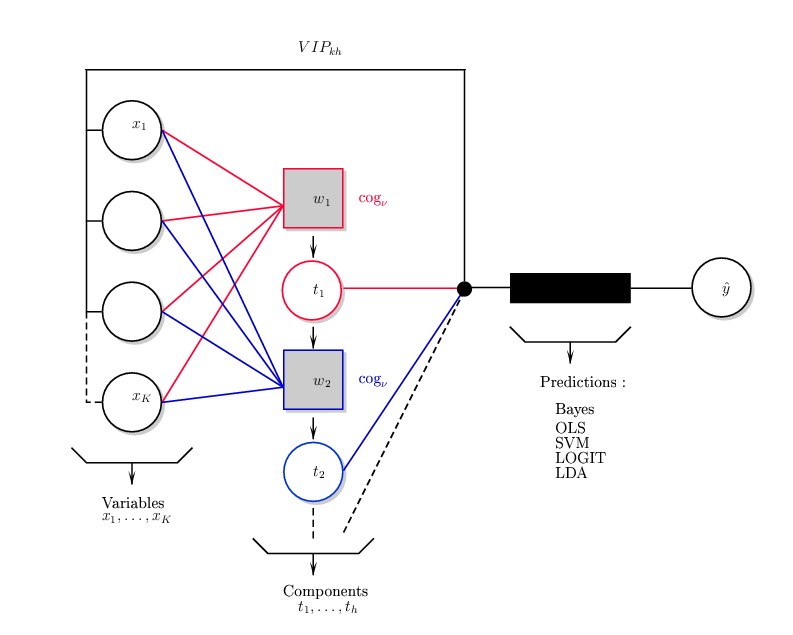
\includegraphics[scale=0.6]{graph.png}
\end{center}


La première étape consiste à trouver des poids de débruitage associés à chaque variable $x_k$ afin d'en déduire la première composante $t_1$ (ou première variable latente). Cette opération est bouclée jusqu'à la composante $t_{h^*}$, où $h^*$ est le nombre optimal de variable latentes. Ainsi, le modèle est estimé :
\begin{equation}\label{forecast}
y=\sum_{h=1}^{h^*} c_ht_h +\eps_h.
\end{equation}   
La statistique $VIP_{hj}$ est mesurée afin de sélectionner la variable $x_j$ qui a l'impact significatif le plus important sur $y$ estimé. Les variables les plus significatives sont celles dont $VIP_{hj}>1$ avec :
\[
VIP_{hj} := \sqrt{\frac{K\sum_{\ell=1}^{h}Rd(y;t_\ell)w_{\ell j}^2}{Rd(y;t_1,\ldots,t_h)}} 
\] 
et 
\[
Rd(y; t_1,\ldots,t_h) := \frac{1}{K}\sum_{\ell=1}^{h}\cor^2(y,t_\ell) =: \sum_{\ell=1}^{h}Rd(y;t_\ell).
\]
où $\text{cor}^2(y,t_\ell)$ est le coefficient de corrélation de Pearson entre $y$ et la composante $t_\ell$. Cette information est rétro-propagée dans le modèle (une seule fois) afin d'obtenir les variables latentes $t_{h^*}$ et leurs coefficients estimés $\hat{c}_{h^*}$ sur les données d'entraînement. La variable cible $y$ est ensuite prédite grâce à (\ref{forecast}). Cette prévision est comparée aux modèles standards SVM, LOGIT, Bayes et LDA lorsque les données tests sont projetées dans le sous-espace $\{t_1,\ldots,t_{h^*}\}$.


\begin{algorithm}[h]
	\small
	\KwResult{ Prédiction du juge $y=0;1$ }
	\Repeat{ $\nu=14$ $[\nu=\nu+2]$ }{
		\Repeat{ $h=10$ $[h=h+1]$ }{
			$\max \cog_\nu(y,w_hX)$ s.t. $\| w_h\|=1$ $\Longrightarrow$ poids $w_h$ de $X$ \;
			MCO équation: $y=\sum_h c_ht_h +\eps_h$ \;
			MCO équation: $R(x_j)=\sum_h \beta_ht_h + \epsilon_k$ $\forall k=1,\ldots,K$ \;
			$X:=(\hat{\epsilon}_1,\ldots,\hat{\epsilon}_K)$ $y:=\hat{\eps}_h$ \; }
		Mesurer $VIP_{kh}$, $Q^2_h$ \;
		Sélectionner le nombre optimal de composantes $h^*$ \; }
	Déduire le paramètre optimal $\nu^*$ qui minimise l'erreur \; 
	\Return Prédiction $\hat{y}$ avec Gini-PLS ($h^*$, $\nu^*$) \;
	\Return Prédiction $\hat{y}$ avec SVM, LOGIT, Bayes, LDA sur les composantes $(t_1,\ldots,t_{h^*})$\;
	\caption{Gini-PLS Généralisé}\label{G-GPLS}
\end{algorithm}
\bigskip

\subsubsection{L'algorithme LOGIT-Gini-PLS généralisé} 
\label{sec:sensresultat:logit-gini-pls}
Comme nous le constatons dans l'algorithme Gini-PLS généralisé que nous avons proposé dans le section précédente, les poids $w_j$ proviennent de l'opérateur co-Gini appliqué à une variable booléenne $y \in \lbrace 0;1 \rbrace$. Afin de trouver les poids $w_j$ qui maximisent le lien entre les variables $x_j$ et la variable cible $y$, nous proposons d'utiliser la régression LOGIT, autrement dit, une sigmoïde qui est mieux adaptée aux variables booléennes. Ainsi, dans chaque étape de la régression Gini-PLS nous remplaçons la maximisation du co-Gini par la mesure de la probabilité conditionnelle suivante :
\begin{equation}\tag{LOGIT}
\mathbb{P}(y_i = 1 / X = X_i) = \frac{\exp\left\{X_i \beta \right\}}{1+\exp\left\{ X_i \beta \right\}}
\end{equation}
où $X_i$ est la $i$-ème ligne de la matrice $X$ (observation des caractéristiques/dimensions de la décision juridique $i$). L'estimation du vecteur $\beta$ se fait par maximum de vraisemblance. On en déduit alors les pondérations $w_j$ :
\[
w_j = \frac{\beta_j}{\| \beta\|}
\]
L'algorithme LOGIT-Gini-PLS généralisé est donc le suivant :

\begin{algorithm}[h]
	\small
	\KwResult{ Prédiction du juge $y=0;1$ }
	\Repeat{ $\nu=14$ $[\nu=\nu+2]$ }{
		\Repeat{ $h=10$ $[h=h+1]$ }{
			LOGIT équation : $\Longrightarrow$ poids $w_j$ de $X$ \;
			MCO équation : $y=\sum_h c_ht_h +\eps_h$ \;
			$X:=(\hat{\epsilon}_1,\ldots,\hat{\epsilon}_K)$ $y:=\hat{\eps}_h$ \; }
		Mesurer $VIP_{kh}$, $Q^2_h$ \;
		Sélectionner le nombre optimal de composantes $h^*$ \; }
	Déduire le paramètre optimal $\nu^*$ qui minimise l'erreur \; 
	\Return Prédiction $\hat{y}$ avec Gini-PLS ($h^*$, $\nu^*$) \;
	\Return Prédiction $\hat{y}$ avec SVM, LOGIT, Bayes, LDA sur les composantes $(t_1,\ldots,t_{h^*})$\;
	\caption{LOGIT-Gini-PLS Généralisé}\label{LG-GPLS}
\end{algorithm}

\section{Expérimentations et résultats}
\label{sec:sensresultat:experimentations}
Nous discutons ici les performances de divers algorithmes populaires et l'impact de la quantité et du déséquilibre des données, de l'heuristique, et de la restriction explicite des documents aux passages relatifs à la catégorie de demandes, ainsi que leur capacité à faire abstraction des autres demandes du document. {Ces expériences visent aussi à comparer l'efficacité du Gini-Logit-PLS par rapport à d'autres analyses discriminantes}.  Comme \citet{im2017textclasstermweighting}, différentes combinaisons d'algorithmes de classification et méthodes de pondération  sont comparées; ce qui représente un total de 8 algorithmes * 11 métriques globales * 5 métriques locales = 440 configurations (+ 2 algorithmes i.e. FastText et NBSVM). La méthode Gini-Logit-PLS réalisant une projection dans un espace de petite dimension, elle a été comparée aussi à d'autres méthode de réduction de dimension.

\subsection{Protocole d'évaluation}
Deux métriques d'évaluation sont utilisées: la précision et la $F_1$-mesure. Pour tenir compte du déséquilibre entre les classes, la moyenne macro est préférée. Il s'agit de l'agrégation de la contribution individuelle de chaque classe: $F_{1macro} = \frac{2 \times P_{macro} \times R_{macro}}{P_{macro} + R_{macro}}$, où les macro-moyennes de la précision ($P_{macro}$) et du rappel ($R_{macro}$) sont calculées en fonction des nombres moyens de vrais positifs ($\overline{TP}$), faux positifs ($\overline{FP}$), et faux négatifs ($\overline{FN}$) comme suit \citep{van2013macromicroeval}:
$P_{macro} = \frac{\overline{TP}}{\overline{TP} + \overline{FP}}$, $R_{macro} = \frac{\overline{TP}}{\overline{TP} + \overline{FN}}$.


Les données utilisées sont une restriction, des données du chapitre précédent, aux documents n'ayant qu'une seule demande annotée pour chacune des catégories de demande. Le déséquilibre entre les classes est illustrée par la figure \ref{fig:sensresultat:stat-1dmd}. En effet, les demandes sont en majorité rejetées pour les catégories ACPA, CONCDEL, DANAIS et STYX. Le contraire est observé pour DCPPC, et le rapport est légèrement équilibré pour DORIS.
\begin{figure}[htb]
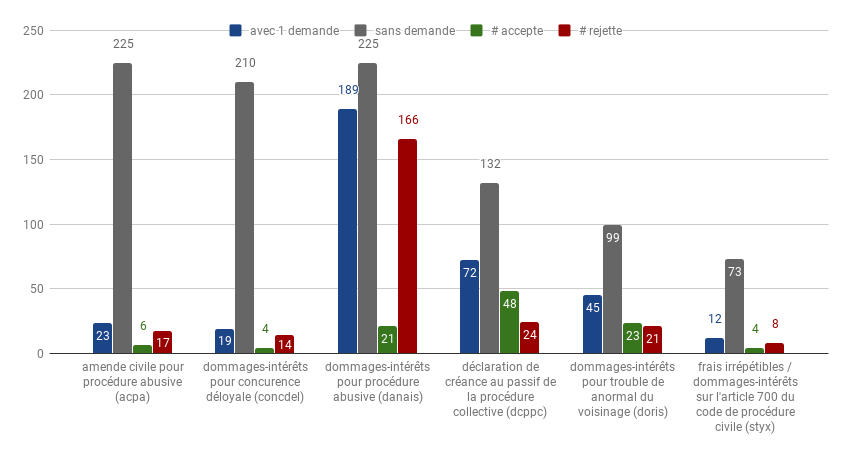
\includegraphics[width=\textwidth]{chartDataset1dmd.png}
\caption{Répartition des documents à une demande de la catégorie considérée.}\label{fig:sensresultat:stat-1dmd}
\end{figure}

L'efficacité des algorithmes dépend souvent des valeurs de méta-paramètres dont il faut déterminer des valeurs optimales. Scikit-learn implémente deux stratégies de recherche des ces valeurs: RandomSearch et GridSearch. Malgré la rapidité de la méthode RandomSearch, elle est non déterministe et les valeurs qu'elle trouve donnent une prédiction moins précise que les valeurs par défaut. Idem pour la méthode GridSearch, qui est très lente, et donc peu pratique face au grand nombre de configurations à évaluer. Par conséquent, les valeurs utilisées pour les expérimentations sont les valeurs par défaut définies par Scikit-learn (Tableau \ref{tab:sensrst:metapara}).

\begin{table}[htb]
	\scriptsize
	\centering
	\begin{tabular}{|l|p{0.7\textwidth}|}
		\hline
		algorithmes & hyper-paramètres\\ \hline
		SVM & $C=1.0; \gamma=\frac{1}{n\_features * var(X)}; noyau=RBF$ (fonction de base radiale)\\ \hline
		KNN & $k = 5, weights='uniform', algorithm='auto'$ \\ \hline
		LDA &  $solver='svd', n\_components=10$\footnote{valeur utilisée pour toutes méthodes de réduction testées}  \\ \hline
		QDA &   \\ \hline
		Arbre & critère de séparation='gini' \\ \hline
		NBSVM & $--ngram=123, linearSVM, $ \\ \hline
		FastText & -minCount=5, -wordNgrams=1, -lr=0.05,    \\ \hline
		Gini-PLS & $h=n\_components=10$ \\ \hline
		Logit-PLS & $h=n\_components=10$  \\ \hline
		Gini-Logit-PLS & $h=n\_components=10; \nu = 14$ \\ \hline
	\end{tabular}
	\caption{Valeurs utilisées pour les méta-paramètres des algorithmes de classification.}\label{tab:sensrst:metapara}
\end{table}

% mu = 14 me semble un peu trop élevé de même  omponents=10=10
%
\subsection{Classification de l'ensemble du document}

En représentant l'ensemble du document à l'aide de diverses représentations vectorielles, les algorithmes sont comparés avec les représentations qui leurs sont optimales. On remarque d'après les résultats du Tableau \ref{tab:sensrst:global} que les arbres sont en moyenne meilleurs sur l'ensemble des catégories même si en moyenne la $F_1$-mesure moyenne est limité à 0.668. Les résultats des extensions du PLS ne sont pas très éloignées de ceux des arbres avec des différences de $F_1$ à moins de 0.1 (si on choisit le bon schéma de "vectorisation").

\begin{table}[!htb]	
	\scriptsize
	
	\textcolor{red}{ajouter les $F_1$ ou erreur de rejette et de accepte}
	
	\textcolor{red}{mettre aussi en avant les analyses discriminantes comme réducteur de dimension et comme classifieurs}
	
	\centering
	\begin{tabular}{|l|l|l|l|l|l|l|l|l|l|}
		\hline
		\textbf{Vecteur} & \textbf{algorithme} & \textbf{$F_1$} & \textbf{min} & \textbf{Cat. min} & \textbf{max} & \textbf{Cat. max} & \textbf{$F_1$ - 1er$F_1$} & \textbf{max - min} & \textbf{rang} \\ \hline
		GSS*TF           & Arbre               & 0.668       & 0.5          & doris             & 0.92         & dcppc             & 0                   & 0.42               & 1             \\ \hline
		AVG-G*TF         & LogitPLS            & 0.648       & 0.518        & danais            & 0.781        & dcppc             & 0.02                & 0.263              & 13            \\ \hline
		AVG-G*TF         & StandardPLS         & 0.636       & 0.49         & danais            & 0.836        & dcppc             & 0.032               & 0.346              & 24            \\ \hline
		DELTADF*TF       & GiniPLS             & 0.586       & 0.411        & danais            & 0.837        & dcppc             & 0.082               & 0.426              & 169           \\ \hline
		DELTADF*TF       & GiniLogitPLS        & 0.578       & 0.225        & styx              & 0.772        & dcppc             & 0.09                & 0.547              & 220           \\ \hline
		-                & NBSVM               & 0.494       & 0.4          & styx              & 0.834        & dcppc             & 0.174               & 0.434              &               \\ \hline
		-                & FastText            & 0.412       & 0.343        & doris             & 0.47         & danais            & 0.256               & 0.127              &               \\ \hline
	\end{tabular}
\caption{Comparaison des algorithmes sur une représentation globale des documents pour la détection du sens du résultat.}\label{tab:sensrst:global}
\end{table}

 Les scores $F_1$ moyens des algorithmes  NBSVM et FastText n'excédent en général pas 0.5 malgré qu'ils soient spécialement conçus pour les textes. On peut estimer qu'ils sont très sensibles au déséquilibre des données entre les catégories (plus de rejets que d'acceptations), soit il est plus difficile de détecter l'acceptation des demandes. En effet, ces algorithmes classent toutes les données test avec le label (sens) majoritaire i.e. le rejet, et par conséquent, ils ne détectent quasiment pas d'acceptation de demande. Le cas des catégories DORIS et DCPPC pour le NBSVM ($F_{1macro} = 0.834$) tend à démontrer la forte sensibilité aux cas négatifs de ces algorithmes puisque même avec presque autant de labels "accepte" que "rejette", la $F_1$-mesure de "rejette" est toujours supérieure à celle de "accepte" (Tableau \ref{tab:sensrst:fasttextnbsvm}). 
 
 \begin{table}[htb]
 	\footnotesize \centering
 	\begin{tabular}{|l|l|l|l|l|l|l|l|l|}
 		\hline
 	\textbf{Cat. Dmd.} & \textbf{Algo.} & \textbf{Préc.}   & \textbf{Préc. équi.} & \textbf{err-0} & \textbf{err-1} & $F_1(0)$  & $F_1(1)$  & \textbf{$F_{1macro}$} \\ \hline
 	\textbf{dcppc}       & nbsvm      & 0.875 & 0.812        & 0.375 & 0     & 0.752 & 0.916 & \textbf{0.834}        \\ \hline
 	danais      & fasttext   & 0.888 & 0.5          & 0     & 1     & 0.941    & 0 & 0.47         \\ \hline
 	danais      & nbsvm      & 0.888 & 0.5          & 0     & 1     & 0.941 & 0     & 0.47         \\ \hline
 	concdel     & fasttext   & 0.775 & 0.5          & 0     & 1     & 0.853     & 0 & 0.437        \\ \hline
 	concdel     & nbsvm      & 0.775 & 0.5          & 0     & 1     & 0.873 & 0     & 0.437        \\ \hline
 	acpa        & fasttext   & 0.745 & 0.5          & 0     & 1     & 0.853     & 0 & 0.426        \\ \hline
 	acpa        & nbsvm      & 0.745 & 0.5          & 0     & 1     & 0.853 & 0     & 0.426        \\ \hline
 	doris       & nbsvm      & 0.5   & 0.492        & 0.85  & 0.167 & 0.174 & 0.63  & 0.402        \\ \hline
 	dcppc       & fasttext   & 0.667 & 0.5          & 1     & 0     & 0.8   & 0     & 0.4          \\ \hline
 	styx        & fasttext   & 0.667 & 0.5          & 1     & 0     & 0.8     & 0   & 0.4          \\ \hline
 	styx        & nbsvm      & 0.667 & 0.5          & 0     & 1     & 0.8   & 0     & 0.4          \\ \hline
 	doris & fasttext & 0.523 & 0.5 & 1 & 0 & 0 & 0.686 & 0.343 \\ \hline
 	\end{tabular}
 	
 $0 == 'accepte'; 1 == 'rejette'$

\caption{Détails des résultats de FastText et NBSVM.}\label{tab:sensrst:fasttextnbsvm}
 \end{table}

\subsection{Réduction du document aux régions comprenant le vocabulaire de la catégorie}
Etant donné que les décisions portent sur plusieurs catégories de demande, nous avons expérimenté la restriction du document aux passages comprenant du vocabulaire de la catégorie d'intérêt: demande, résultat, résultat antérieur (resultat\_a), paragraphes dans les motifs (motifs). Les combinaisons passages-représentation vectorielle-algorithme sont comparées dans le Tableau \ref{tab:sensrst:zone}. Les résultats s'améliorent énormément avec les réductions, sauf pour la catégorie DORIS. La meilleure restriction combine les passages comprenant le vocabulaire de la catégorie dans la section Litige (demande et résultat antérieur),  dans la section Motifs (contexte), et dans la section Dispositif (résultat).
\begin{table}[!htb]
	\scriptsize
	\centering
	
	\begin{tabular}{|l|l|l|l|l|}
		\hline
		\textbf{Catégorie} & \textbf{zone}                                    & \textbf{Vecteur (pondération)}      & \textbf{classifieur} & $F_1$    \\ \hline
		\multirow{3}{*}{acpa}    & \textbf{demande\_resultat\_a\_resultat\_context} & \textbf{DBIDF*TF}           & \textbf{Tree}        & \textbf{0.846} \\ 
		              & litige\_motifs\_dispositif                       & DELTADF*TF                  & StandardPLS       & 0.697          \\ 
		              & litige\_motifs\_dispositif                       & AVERAGEGlobals*TF           & LogitPLS          & 0.683          \\ \hline
		\multirow{3}{*}{concdel}  & \textbf{litige\_motifs\_dispositif}              & \textbf{GSS*TF}             & \textbf{Tree}        & \textbf{0.798} \\ 
		           & motifs                                           & IDF*TF                      & GiniLogitPLS      & 0.703          \\ 
		           & context                                          & DBIDF*LOGAVE                & StandardPLS       & 0.657          \\ \hline
		\multirow{3}{*}{danais}   & \textbf{demande\_resultat\_a\_resultat\_context} & \textbf{CHI2*AVERAGELocals} & \textbf{Tree}        & \textbf{0.813} \\ 
		            & demande\_resultat\_a\_resultat\_context          & AVERAGEGlobals*ATF          & LogitPLS          & 0.721          \\ 
		            & demande\_resultat\_a\_resultat\_context          & AVERAGEGlobals*ATF          & StandardPLS       & 0.695          \\ \hline
		\multirow{3}{*}{dcppc}    & \textbf{demande\_resultat\_a\_resultat\_context} & \textbf{CHI2*TF}            & \textbf{Tree}        & \textbf{0.985} \\ 
		             & demande\_resultat\_a\_resultat\_context          & CHI2*TF                     & LogitPLS          & 0.94           \\ 
		             & litige\_motifs\_dispositif                       & MARASCUILO*TP               & StandardPLS       & 0.934          \\ \hline
		\multirow{3}{*}{doris}    & \textbf{litige\_motifs\_dispositif}              & \textbf{DSIDF*TP}           & \textbf{GiniPLS}  & \textbf{0.806} \\
		             & litige\_motifs\_dispositif                       & DSIDF*TP                    & GiniLogitPLS      & 0.806          \\
		             & litige\_motifs\_dispositif                       & IG*ATF                      & StandardPLS       & 0.772          \\ \hline
		\multirow{3}{*}{styx}     & \textbf{motifs}                                  & \textbf{DSIDF*TF}           & \textbf{Tree}        & \textbf{1}     \\ 
		             & demande\_resultat\_a\_resultat\_context          & DSIDF*LOGAVE                & GiniLogitPLS      & 0.917          \\ 
		              & litige\_motifs\_dispositif                       & RF*TF                       & GiniPLS           & 0.833          \\ \hline
	\end{tabular}
\caption{Détection du sens du résultat: Comparaison des réductions du document.}\label{tab:sensrst:zone}
\end{table}

\section{Conclusion}
\label{sec:sensresultat:conclusion}
L'étude de ce chapitre tente de simplifier l'extraction du sens du résultat rendu par les juges sur une demande de catégorie donnée. Elle a consisté à formuler le problème comme une tâche de classification de documents. On évite ainsi de passer par la détection ad-hoc\footnote{i.e. spécialement conçu pour nos données.} des passages et données à l'aide de termes-clés qui est un inconvénient de la méthode à règles du chapitre précédent car elle n'est peut-être pas généralisable à tous types de décisions (i.e. il pourrait être nécessaire d'établir de nouvelles listes de mots-clés pour d'autres domaines). Au total dix algorithmes de classification on été expérimentés sur 55 méthodes de représentations vectorielles de texte. Nous avons remarqué que les résultats de classification sont principalement influencés par 3 caractéristiques de nos données. Tout d'abord, le très faible nombre d'exemples d'entraînement défavorise certains algorithmes (sensibilité aux valeurs aberrantes ou \textit{outliers}), comme par exemple FastText qui nécessite plusieurs milliers d'exemples pour mettre à jour le pas du gradient (\textit{learning rate}). Ensuite, le fort déséquilibre entre les classes ("accepte" vs. "rejette") rend difficile la reconnaissance de la classe minoritaire qui est généralement la classe "accepte". Le fort gap entre les erreurs sur "rejette" et celles sur "accepte", ainsi que les bons résultats obtenus sur DCPPC en sont la preuve. Enfin, la présence d'autres catégories de demande dans le document dégrade l'efficacité de la classification parce que les algorithmes ne parviennent pas seuls à retrouver les éléments en rapport direct avec la catégorie choisie. Ceci est démontré par l'impact positif de la restriction du contenu à classer à certains passages particuliers, même si la restriction adéquate est fonction de la catégorie.
 
Au final, les arbres de décision sont adaptés pour la tâche, mais l'usage du Gini-PLS et du Gini-Logit-PLS permet d'obtenir des performances assez proches de celles des arbres. %??? comparaison avec d'autres analyses discriminantes ???.
Il serait intéressant de combiner ces variantes de l'analyse PLS, à d'autres comme le Sparse-PLS qui pourrait peut-être aider à résoudre le problème de vecteurs/matrices creuses dont sont victimes les représentations vectorielles de texte. Il existe aussi un grand nombre d'architectures neuronales pour la classification de document et de très grands nombres de métriques de pondération de termes pour la représentation des textes, mais aucune ne semble s'adapter à toutes les catégories. Par conséquent, une étude sur l'usage des représentations par plongement sémantique comme Word2Vec \citep{mikolov2013word2vec}, Sent2Vec \citep{pagliardini2017sent2vec} ou Doc2Vec \citep{quoc2014doc2vec} serait intéressante.
